%****************************************************
%	CHAPTER 1 - INTRODUCTION
%****************************************************
\chapter{Introduction}
\label{ch:introduction}
%====================================================
\section{Background}
\label{sec:ch1.background}
%====================================================
\subsection{Subsection}
\label{subsec:ch1.section1.subsec1}
%----------------------------------------------------
In ullamcorper blandit quam. Sed tortor felis, mattis at, pretium et, tempus sit amet, pede. Mauris laoreet scelerisque dui. Curabitur eu risus. Aliquam gravida vehicula erat. Pellentesque suscipit ultricies dui. Aliquam faucibus sagittis felis. Nulla enim. Nulla facilisi. Sed non purus luctus magna bibendum pretium. Aliquam egestas mattis sapien. Duis laoreet nisl at est.
Integer at massa. Duis ut sapien sit amet ipsum pretium eleifend. Vivamus augue ante, pretium non, ornare ac, egestas non, lectus. Phasellus tristique. Nullam nec quam id neque pellentesque ornare. Maecenas semper elit id dui.
Fusce libero urna, porttitor a, molestie in, vestibulum sit amet, enim. Morbi facilisis nulla at purus elementum pharetra. Proin malesuada, odio eu tempus posuere, diam justo consequat.\footnote{This is a footnote}
%====================================================
\subsubsection{Sub-subsection}
\label{subsec:ch1.section1.subsubsec1}
%----------------------------------------------------
\begin{figure}[H]
    \centering
    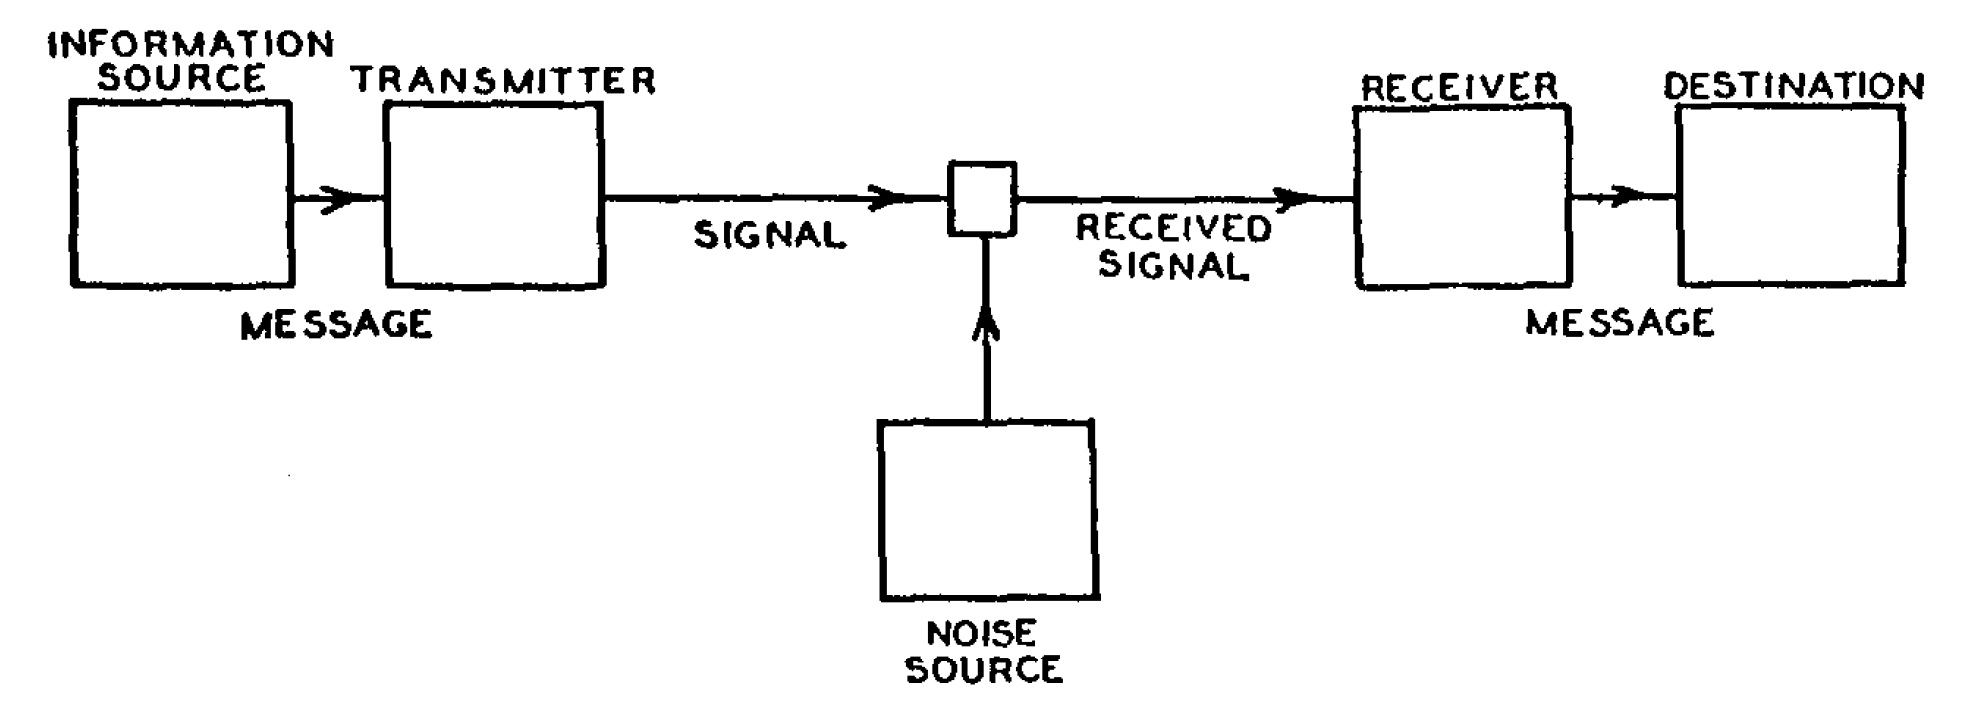
\includegraphics[width=0.8\textwidth]{figs/ch1/shannon.jpg}
\caption[A simplified block diagram of a general communication system.]{\textbf{A simplified block diagram of a general communication system.} A communication system can be abstracted as follows: an \textit{information source} produces a message to be sent through a \textit{transmitter} which converts it to a signal which can be sent via a communication \textit{channel}. The received signal is noisy and is converted back to the message by the \textit{receiver} which is then delivered to the \textit{destination}. Taken from \cite{shannon1948}.}
    \label{fig:my_label}
\end{figure}
%----------------------------------------------------
\pagebreak
%----------------------------------------------------
\begin{table}[H]
    \centering
    \caption[Table title]{\textbf{Table title.} Extended description of tables contents.}
    \begin{tabularx}{\textwidth}{>{\raggedright\arraybackslash}m{8cm}>{\raggedright\arraybackslash}X>{\raggedright\arraybackslash}X}
    \toprule[2.25pt]
    \multirow{3}{*}{\textbf{Heading 1}}        &  \multicolumn{2}{c}{\textbf{Heading 2}}   \\
    \cmidrule[0.5pt](lr){2-3}
    &  \multicolumn{1}{c}{\textit{\small Subheading 1}} & \multicolumn{1}{c}{\small \textit{Subheading 2}}\\
    &  \multicolumn{1}{c}{\small [units]} & \multicolumn{1}{c}{\small [units]}\\
    \midrule[1pt]
         &  &\\
         &  &\\
         &  &\\
    \bottomrule[2.25pt]
 \end{tabularx}

    \label{table:my_label}
\end{table}


%====================================================
\section{Problem statement}
\label{sec:ch1.problemstatement}
%====================================================
Equations are numbered and include the chapter number. As they are considered part of the text, they include punctuation, and each parameter must be described in the text below. Ensure that the units are stated and where possible use SI units. For example, the Maxwell equations are expressed as:
\begin{align}
\nabla \cdot \bm{E} &= \frac{\rho}{\epsilon_0}, \\
\nabla \cdot \bm{B} &= 0, \\
\nabla \times \bm{E} &= -\frac{\partial \bm{B}}{\partial t}, \\
\nabla \times \bm{B} &= \mu_0 \bm{J} + \mu_0 \epsilon_0 \frac{\partial \bm{E}}{\partial t},
\end{align}

where $\bm{B}$ is the magnetic flux density in T, $\bm{J}$ is the total current density in A/m$^2$, $\bm{E}$ is the electric field in V/m, $\mu_0$ is the permeability of free space (4\(\pi \times 10^{-7}\) H/m), and $\epsilon_0$ is the permittivity of free space (8.85 \(\times 10^{-12}\) C$^2$/N·m$^2$).


%====================================================
\section{Project objectives}
\label{sec:ch1.projectobjectives}
%====================================================
The \gls{gps} is used for positioning. The \gls{miz} is of particular interest in the \gls{so}.
%====================================================
\section{Scope, limitations and assumptions}
\label{sec:ch1.scope}
%====================================================
%====================================================
\section{Plan of development}
\label{sec:ch1.planofdevelopment}
\pagebreak
%====================================================
%----------------------------------------------------
%****************************************************
% END
%****************************************************
